\section{Our Model}
As mentioned in the introduction, we investigate our basic model: segregation of $20$ individuals of type $1$ and $20$ individuals of type $2$ on a $8 \times 8$ board.
In this model an individual moves if less than one third of his/her neighbours is not of his/her type to the nearest place where he/she becomes happier.
Every person without neighbours is by definition unhappy (so his/her happiness is $0$), because nobody wants to be alone.
Furthermore, the basic model uses the second order neighbourhood: so the maximum number of neighbours is eight.\\

First of all, we can change the size of the board.
Without changing any other parameters, this only implies that the board becomes busier or more quiet.
Secondly, we can also change the number of different types on the board.
For instance, we can look at a $12\times 12$ board with $10$ types of individuals and $10$ individuals per type: see figure \ref{fig:example big board}.
As one can see, far more individuals have been moved to another place on the board and they form groups.

\begin{figure}[H]
	\centering
    \begin{subfigure}{0.45\textwidth}
        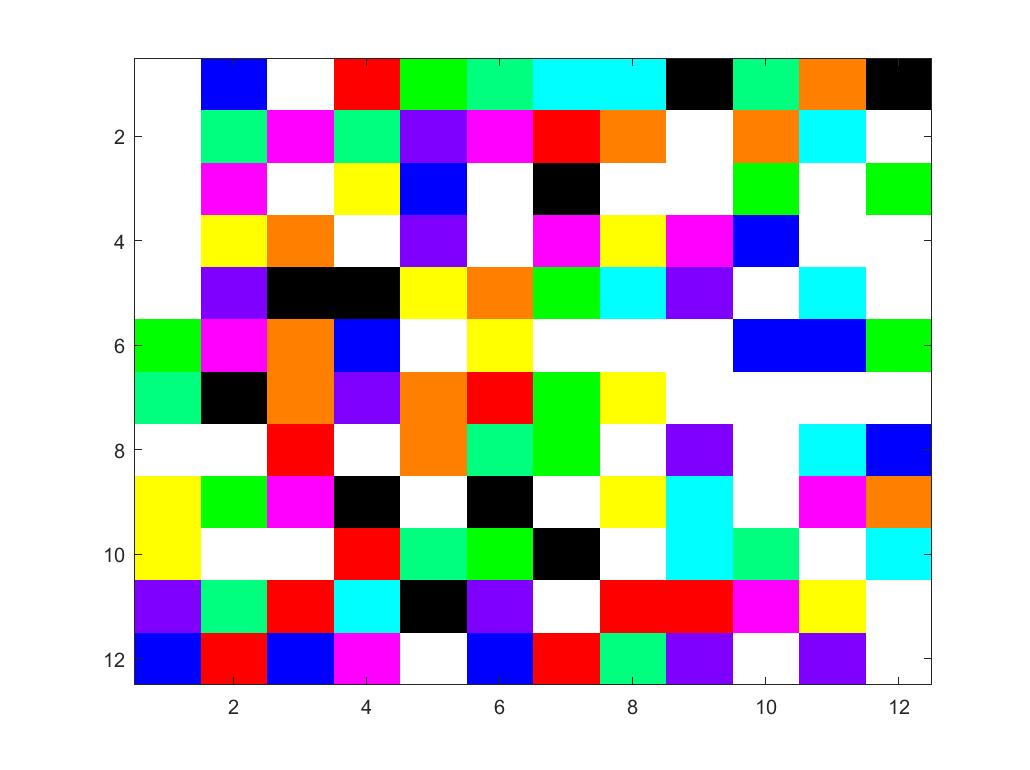
\includegraphics[width=\textwidth]{vb2beginbord.jpg}
        \caption{Situation before segregation}
        \label{fig:example big board begin}
    \end{subfigure}\hspace{0cm}
    ~ 
    \begin{subfigure}{0.45\textwidth}
        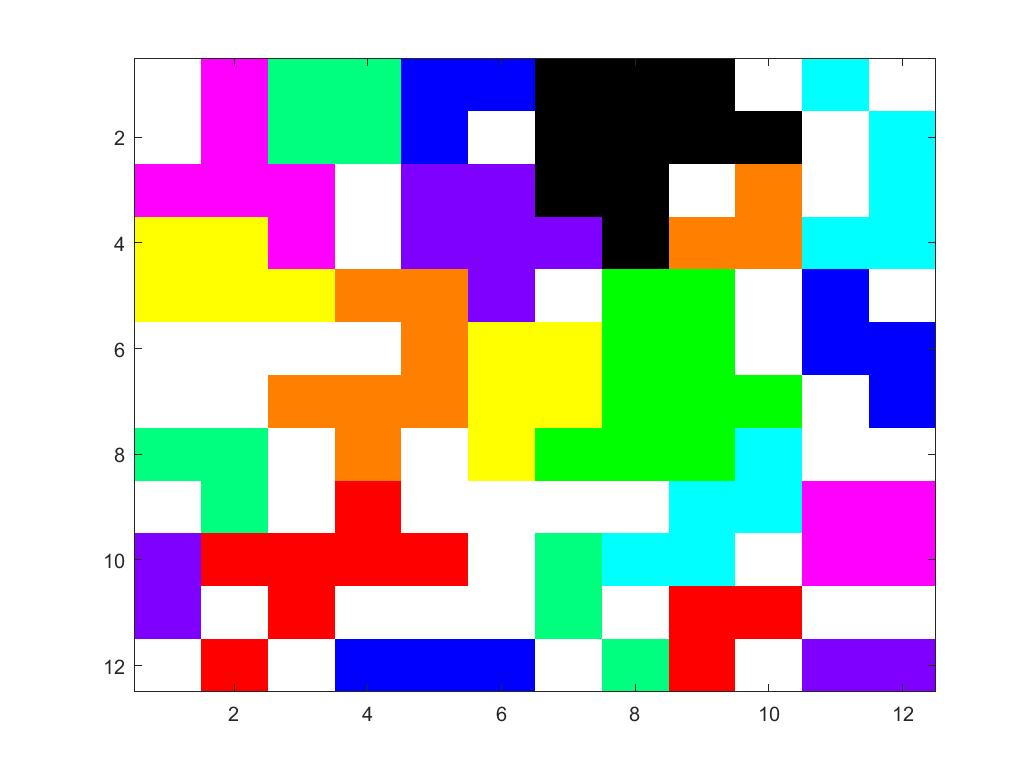
\includegraphics[width=\textwidth]{vb2eindbord.jpg}
        \caption{Situation after segregation}
        \label{fig:example big board end}
    \end{subfigure}
    ~ 
    \caption{An example of segregation in a model on a $12\times 12$ board with $100$ individual of $10$ different types}
    \label{fig:example big board}
\end{figure}

Subsesquently, we can vary our 'happinessrule': the minimum fraction of neighbours of an individuals own type to be happy.
Our expectation is that it takes longer to reach equilibrium if the happinessrule is higher.
This seems logic, since all individuals want to be surrounded by relatively more neighbours of their own type.
In consequence, larger homogenous groups will be formed after segregation with a higher happinessrule.
In figure \ref{fig:examplehap2/3} and \ref{fig:examplehap1} we can see what the effect is of a happiness rule of respectively $\frac{2}{3}$ and $1$ on the board after segregation.

\begin{figure}[H]
	\centering
    \begin{subfigure}{0.4\textwidth}
        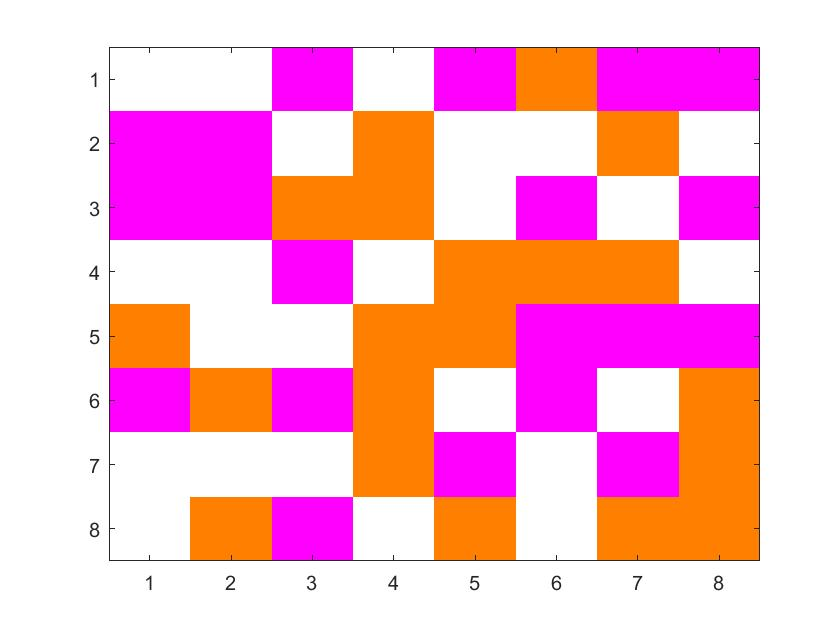
\includegraphics[width=\textwidth]{vb3beginbord.jpg}
        \caption{Situation before segregation}
        \label{fig:example hap 2/3 begin}
    \end{subfigure}\hspace{0cm}
    ~ 
    \begin{subfigure}{0.4\textwidth}
        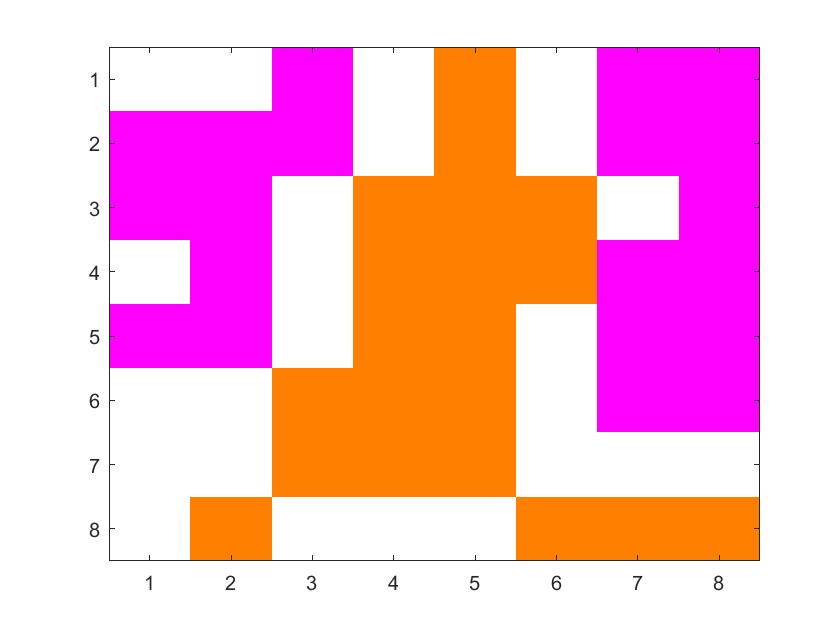
\includegraphics[width=\textwidth]{vb3eindbord.jpg}
        \caption{Situation after segregation}
        \label{fig:example hap 2/3 end}
    \end{subfigure}
    ~ 
    \caption{An example of segregation in a model with happinessrule $\frac{2}{3}$}
    \label{fig:examplehap2/3}
\end{figure}

\begin{figure}[H]
	\centering
    \begin{subfigure}{0.4\textwidth}
        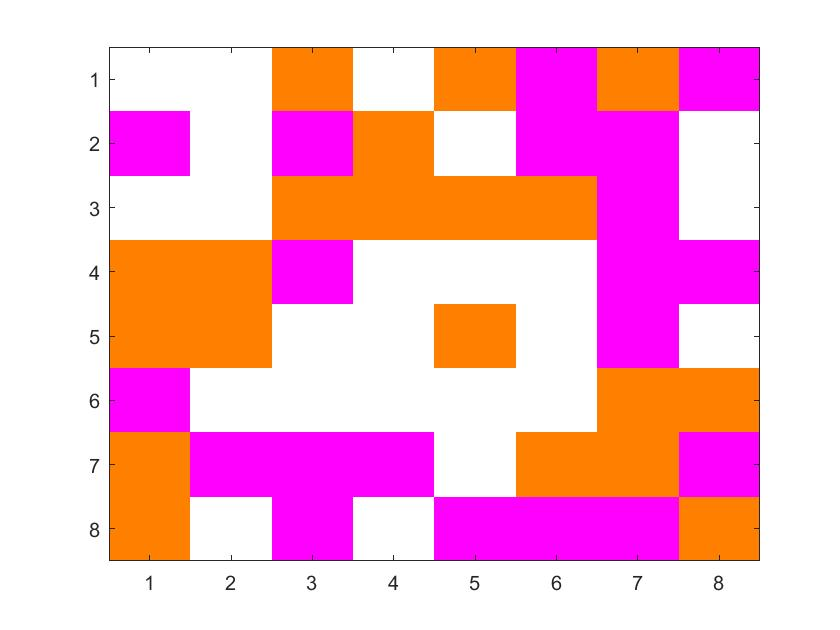
\includegraphics[width=\textwidth]{vb4beginbord.jpg}
        \caption{Situation before segregation}
        \label{fig:example hap 1 begin}
    \end{subfigure}\hspace{0cm}
    ~ 
    \begin{subfigure}{0.4\textwidth}
        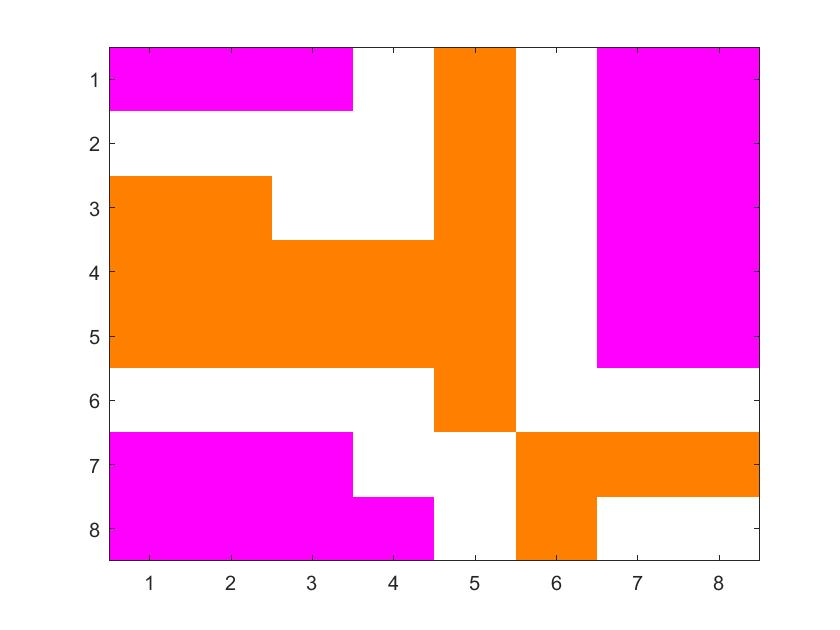
\includegraphics[width=\textwidth]{vb4eindbord.jpg}
        \caption{Situation after segregation}
        \label{fig:example hap 1 end}
    \end{subfigure}
    ~ 
    \caption{An example of segregation in a model with happinessrule $1$}
    \label{fig:examplehap1}
\end{figure}

%We can see that in figure \ref{fig:example hap 1 end} every individual has only neighbours of their own type due to the happinessrule of $1$.
%We will elaborate on the influence of the happinessrule on the model in section $4$ and $5$.\\

\begin{wrapfigure}{r}{0.3\textwidth}
\vspace{-20pt}
\centering
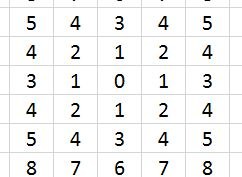
\includegraphics[scale=0.5]{buurtorde.jpg}
\caption{Neighbourhoodorder}
\vspace{-15pt}
\label{fig:neighbourhood}
\end{wrapfigure}

In addition, we are able to change the type of neighbourhood.
The standardtype of neighbourhood is the second: in this case every individual can have up to eight neighbours.
There exists one smaller type of neighbourhoods: the first type of neighbourhood, where everybody has up to four neighbours.
The best way to show how the bigger types of neighbourhood are formed is figure \ref{fig:neighbourhood}.
Here is the $0$ an individual and for every other place is the number the smaller order of neighbourhood of that individual that contains that place.
We will not research the influence of the type of neighbourhood on the segregation in our model in our report.
However, we added some interesting graphs in our appendix.\\

Moreover, we included the possibility for individuals to a random place on the board if he/she is not happy.
In the basic model he/she will move to the nearest place where he/she will become happier, so we expect that with the random move it takes longer to reach an equilibrium.
Again, we will not discuss the impact of the random move in our report, but added some nice results in our appendix.\\

Furthermore, we expanded the model with the so-called 'criminals'.
It is possible to call $c$ of the $n$ individuals a criminal.
Everybody who is not a criminal does not like criminals, so their happiness is $0$ if a criminal is in their neighbourhood.
As a result, all criminals should end up together after segregation.
In figure \ref{fig:examplecrim}, one can see an example of the basic model with $10$ criminals among the $40$ individuals.
It is visible that our expactation is not always true.
In this case, equilibrium is reached, because every unhappy individual could not move to another place as a consequence of the fact that every empty place in a neighbourhood of a criminal or in no one's neighbourhood.
So the unhappy individuals will not become happier on these places.

\begin{figure}[H]
	\centering
    \begin{subfigure}{0.4\textwidth}
        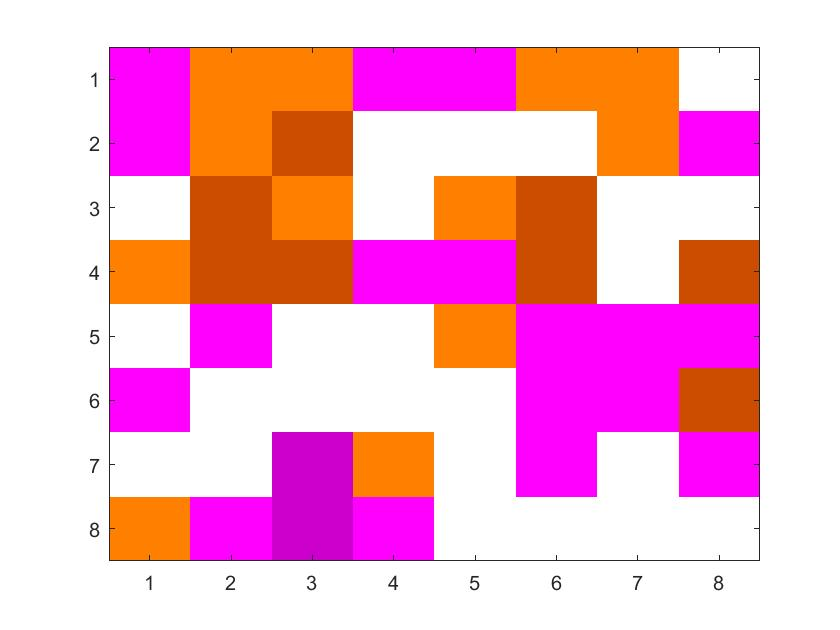
\includegraphics[width=\textwidth]{vb5beginbord.jpg}
        \caption{Situation before segregation}
        \label{fig:example crim begin}
    \end{subfigure}\hspace{0cm}
    ~ 
    \begin{subfigure}{0.4\textwidth}
        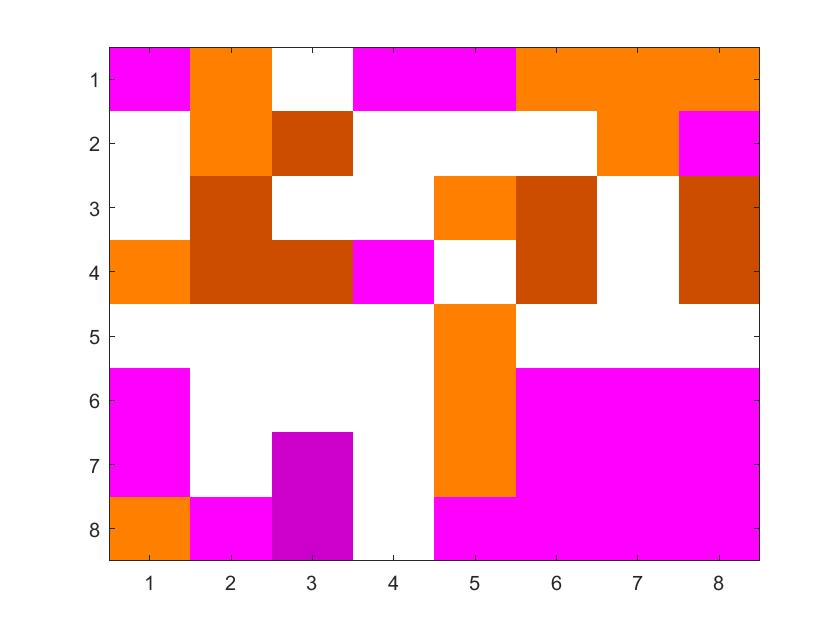
\includegraphics[width=\textwidth]{vb5eindbord.jpg}
        \caption{Situation after segregation}
        \label{fig:example crim end}
    \end{subfigure}
    ~ 
    \caption{An example of segregation in the basic model with $10$ criminals (the slightly darker places)}
    \label{fig:examplecrim}
\end{figure}

Last but not least, we made it possible for individuals to switch to another type.
In our model there are two types of switching.
The first is only possible if there are only individuals of type $1$ and type $2$.
In this version of switching, every person has in every generation a chance $p$ to become of the other type.
In the other version, every unhappy individual will change type under influence of his/her neighbours.
This means that the chance to become of type $t$ is the fraction of neighbours of type $t$.
This is a correct probability distribution, because this sums up to $1$.
Individuals without neighbours will not switch type, because they have no neighbours who influence them.
We will investigate the influence of the second type of switching further in section $7$.


